\documentclass[10pt,conference,compsocconf]{IEEEtran}

%\usepackage{times}
%\usepackage{balance}
\usepackage{url}
\usepackage{graphicx}	% For figure environment
\usepackage{xcolor}
\usepackage{array}% http://ctan.org/pkg/array
\usepackage[inline]{enumitem}
\usepackage{caption}
\usepackage{subcaption}
\usepackage{tikz}

\usetikzlibrary{positioning}
\usetikzlibrary{calc}

\newcommand{\lh}[1] {
  \textcolor{blue}{Lucas: #1}}
  
  
\newcommand{\blue}[1] {
  \textcolor{blue}{#1}}
  
\newcommand{\sam}[1] {
  \textcolor{green}{Sam: #1}}

\begin{document}
\title{Leveraging Transformers for Road Segmentation}

\author{
  Samuel Bedassa Alemu, Robin Bisping, Lucas Habersaat \textit{(Group: Rosas)}\\
  Computational Intelligence Lab, Department of Computer Science, ETH Zurich, Switzerland
}

\maketitle

\begin{abstract}
Following the success in medical segmentation, we leverage transformers for segmenting aerial images. Transformers compensate the weaknesses of UNets and improve classification. In particular, we use several state-of-the-art transformer-based UNet architectures, the most promising being TransUNet along with various pre- and post-processing methods. We demonstrate a viable approach to apply the attention mechanism to road segmentation tasks.

\end{abstract}

\section{Introduction}

Images contain a great deal of information, their processing and interpretation is a crucial task in many fields. Image segmentation is a feature extraction problem, i.e., the process of assigning each pixel or patch of pixels in an image to a particular category. This ultimately divides the image into distinct regions. This process creates a simplified representation of an image that is more informative for analysis than images, which are inherently high-dimensional.

Machine learning has revisited this topic and provided many new solutions to current problems in interpreting visual data. In the case of road segmentation, each pixel of an RGB aerial image is assigned the label \textit{road} or \textit{non-road}. In formulating our solution to this problem, we considered several architectural approaches to improve our prediction accuracy and generalization. Our novel approach leverages recent developments in medical segmentation, combining transformers with CNN architectures.


\subsection{Problem Description}
The given problem is to segment aerial images from Google Maps into road pixels and non-road pixels. The course provided two data sets for training and testing purposes. Training data of 100 images with a resolution of $400 \times 400$ with ground truth labels assigning each pixel the value $1$ if it is a road and $0$ if not, and a test set of 94 images with a resolution of $608 \times 608$. To evaluate the classifier, the proportion of correctly predicted patches is measured and used as a score.

\subsection{Related Work}


With the advent of neural networks, new state-of-the-art methods for solving known and new problems have emerged. Driven by these developments, image segmentation is being applied in various fields and several techniques are being developed \cite{PAL19931277}. In the field of aerial imagery, neural networks have also been used to segment images into meaningful urban regions such as streets or buildings \cite{DBLP:journals/corr/abs-2007-06102} \cite{Marmanis2016} \cite{GUPTA202122}.


Along with the recent developments in the field of neural networks, the quality and quantity of data have also taken on new importance. One of the biggest challenges in this area is the lack of training data and its quality. Either labelling must be done by hand and is therefore tedious, or advanced methods must be applied to deal with noisy data \cite{10.5555/3042573.3042603}. A comprehensive review compares many state-of-the-art segmentation methods using a fine-grained and highly detailed data set \cite{DBLP:journals/corr/abs-2007-06102}.


Transformers \cite{Vaswani2017}, that are initially used for sequence modeling and transduction problems, have been applied to image segmentation, as well. In medical segmentation, where for example CT scans must be segmented into regions of organs, Transformers have been successfully applied by combining them with CNNs \cite{Petit2021} \cite{Chen2021}.

\subsection{Contributions}

We combine Transformers and UNets to introduce the Attention-Mechanism to the problem of road segmentation. Together with different pre- and post-processing methods and an automated hyperparameter tuning process, we sought to improve the prediction results.

\section{Models \& Method}

\begin{figure*}[tbp]
  \centering
  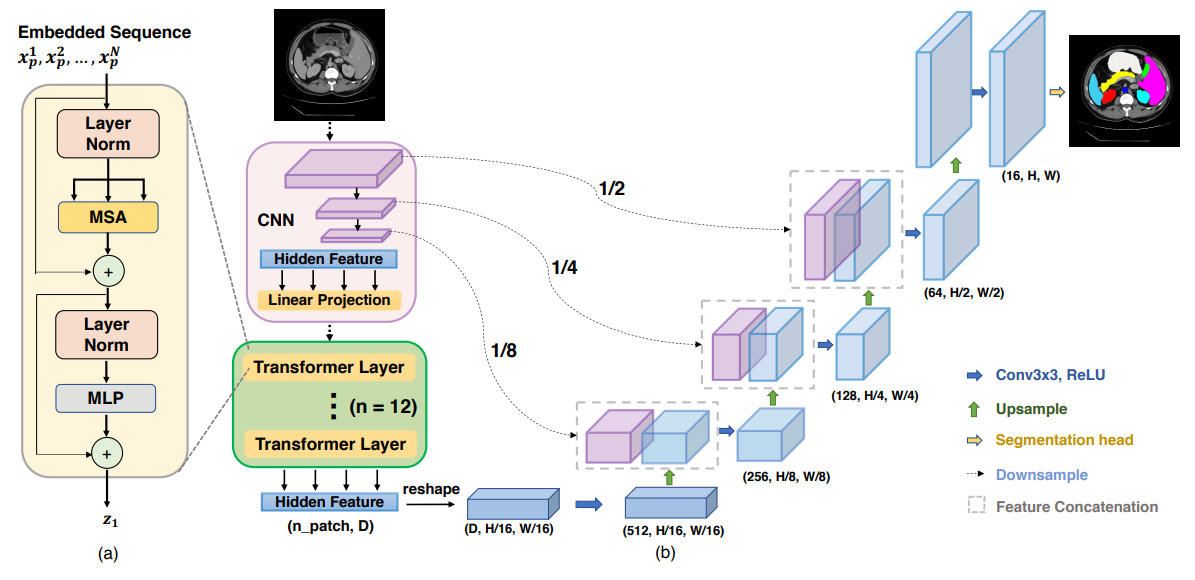
\includegraphics[scale=0.45]{images/trans_unet_model.png}
  \caption{TransUNet - model architecture by Chen et al. (2021). The architecture of the TransUNet resembling a UNet with (a) a hybrid CNN and Transformer encoder, with a stack of $n=12$ Transformer layers; and (b) a cascaded upsampler as decoder with intermediate skip connection.}
  \label{fig:trans_unet_model}
\end{figure*}

\subsection{Background Transformers}

By leveraging Transformers and their success in image segmentation as well as in other domains, we combined Transformers with UNets to compensate for each other's weaknesses. CNNs tend not to model global or long-range dependencies well and are not good at finding contextual interactions. This is due to the intrinsically local nature of the convolution operation. Transformers, on the other hand, can compensate for this drawback by introducing a global context.

\subsubsection{Transformer Model}
In general, Transformers are based on the attention mechanism \cite{Vaswani2017} and have a a classic encoder-decoder structure where each consists of a stack of equal layers. \textbf{\textbf{}} Each layer in the encoder consists of a multi-head self-attention mechanism, see \ref{sec:attention} section, and a simple positional, fully connected feed-forward network. The decoder layer has an additional block that incorporates the output of an encoder layer into a multi-head attention block. After each block, a residual connection ~\cite{7780459} is put around, followed by layer normalization.


% \begin{figure}[tbp]
%   \centering
%   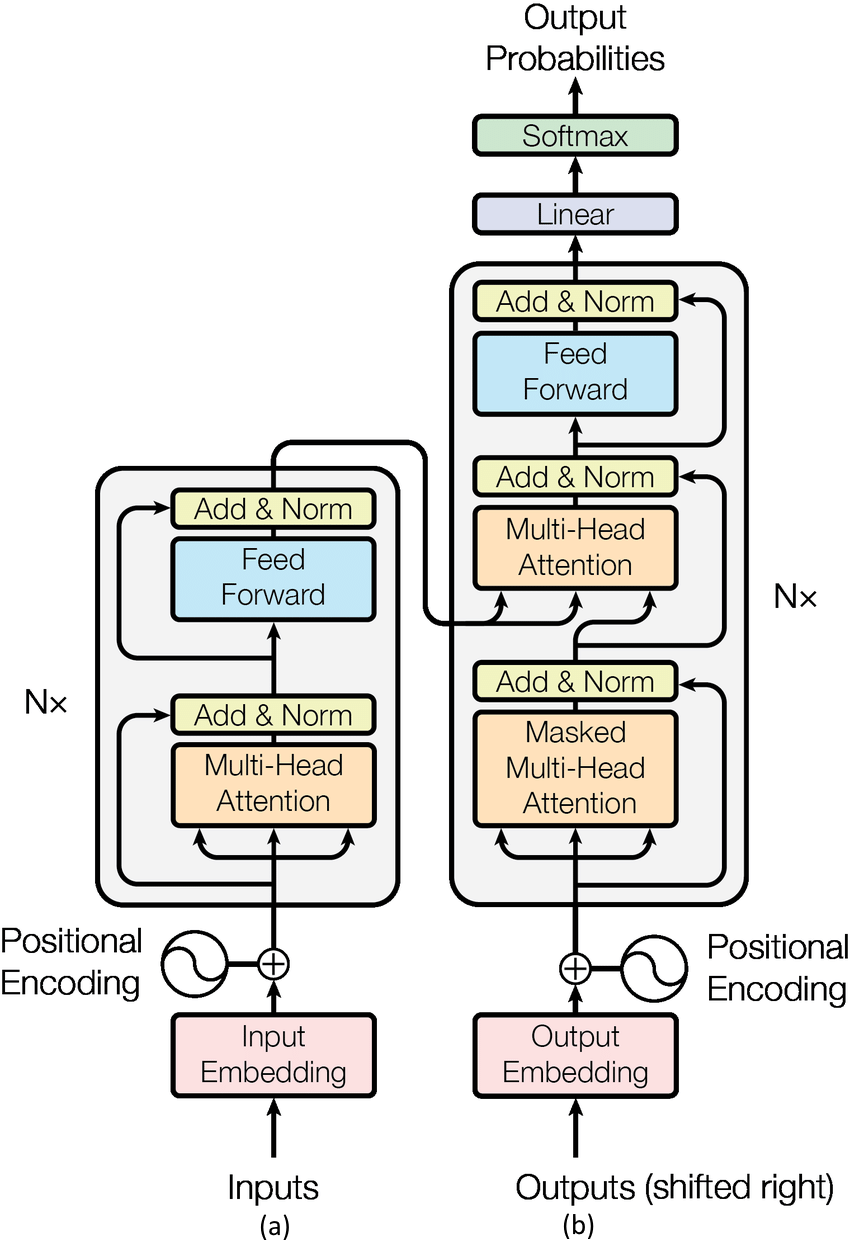
\includegraphics[scale=0.2]{images/transformer_model.png}
%   \caption{The Transformer - model architecture by Vaswani et al. (2017). Left side: encoder. Right side: decoder.   \lh{either omit figure, trim it, and extend label}}
%   \label{fig:transformer_model}
% \end{figure}

\subsubsection{Attention Mechanism}
\label{sec:attention}

\textbf{Self-attention} is an attention mechanism that attempts to discover patterns among inputs in a single input sequence, it resembles the human reading process. It boils down to the Function \ref{eqn:attention_function}that maps queries and key-value pairs to output. The queries $Q$, keys $K$ and values $V$ are derived from the input with trained weights.

\begin{equation}
    A=softmax(\frac{QK^T}{\sqrt{d_k}})
    \label{eqn:attention_function}
\end{equation}

where $d_k$ is the dimension of queries and keys. In the attention matrix $A$, a row corresponds to the similarity of an element in $Q$ with regard to all elements in $K$ \cite{Vaswani2017}. This mechanism connects all elements with each other and global context is incorporated in this way.

\textbf{Multi-head} self-attention runs the attention mechanism $h$ times in parallel using different projections for the queries, keys and values and at the end concatenates and projects the values back into the final output.

\subsection{TransUNet}
The architecture used is mainly based on the TransUNet \cite{Chen2021} model that has introduced a new state-of-the-art method for medical applications. It has a classic encoder-decoder structure and combines Transformers and their attention mechanism with a UNet. The \textbf{encoder} part consists of a hybrid setup of a CNN and a Transformer. The CNN first extract features for the Transformer to further interpret. This also allows feature aggregation of intermediate feature maps using skip-connections. The Transformer part consists of $n=12$ equal Transformer layers. They are identical to the Transformer stack from \cite{Vaswani2017}, a multi-head attention block and a multi-layer perceptron block, each followed by layer-normalization. The \textbf{decoder} resembles the UNet decoder and upsamples the hidden features in a cascaded manner to the full resolution again. Each upsampling step consists of a doubling upsampling operator, a $3\times 3$ convolution layer and a ReLU layer. Additional skip-connections aggregate features at all resolution levels. The exact and detailed architecture can be observed in Figure \ref{fig:trans_unet_model}.

\subsection{Pre-Processing}

The provided dataset poses several challenges:
\begin{enumerate*}[label=(\arabic*)]
  \item It consists of only 100 images. This is a relatively small amount of data.
  \item Using full-sized images can exceed the computational resources of common hardware. In particular, the memory available on usual graphic cards does not suffice to train the UNet Transformer architecture \cite{Petit2021} with images of size $400\times 400$.
  \item The test dataset consists of images of a different size than the training dataset. This makes transformations necessary.
\end{enumerate*} 

In order to counter the shortcomings of the dataset, we introduce several pre- and post-processing steps into our pipeline.

\begin{figure}[h]
    \centering
    
    \begin{tikzpicture}
        \tikzstyle{arrow}=[->,rounded corners,line width=1pt]
        \tikzstyle{label}=[shape=circle,draw,fill=white,inner sep=1.5pt]
    
        \node (original) at (0, 0) {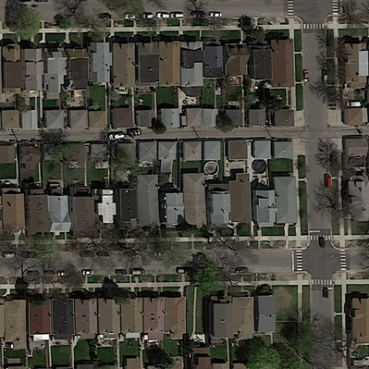
\includegraphics[width=.3\columnwidth]{images/original.png}};
        \node (enhanced) at (4.5, 0) {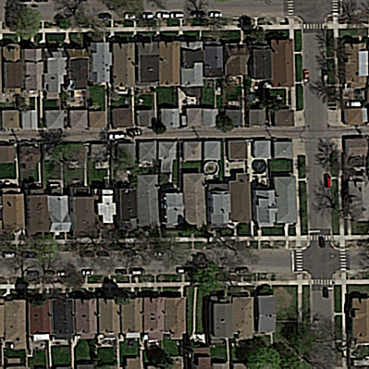
\includegraphics[width=.3\columnwidth]{images/enhanced.png}};
        \node (crop1) at (1, -3) {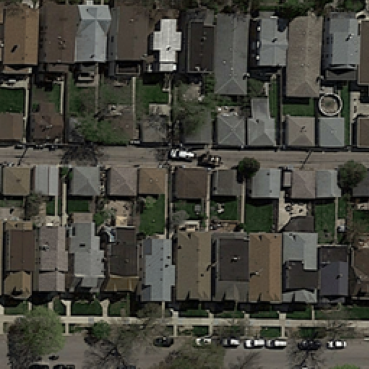
\includegraphics[width=.2\columnwidth]{images/crop1.png}};
        \node (crop2) at (3.25, -3) {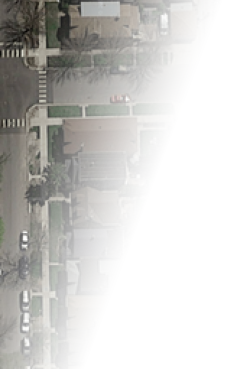
\includegraphics[height=.2\columnwidth]{images/crop2_gradient.png}};
        \node (crop3) at (5, -3) {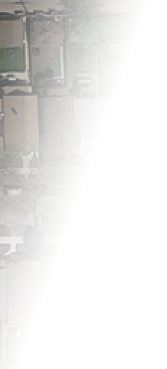
\includegraphics[height=.2\columnwidth]{images/crop3_gradient.png}};
        \node (noise) at (-0.5, -5.5) {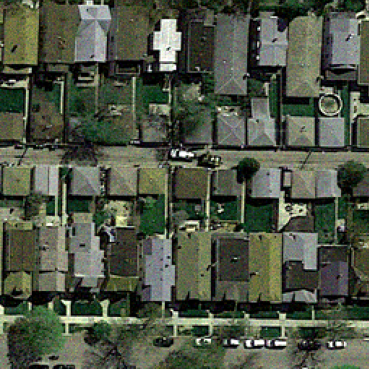
\includegraphics[width=.2\columnwidth]{images/noise.png}};
        \node (centered) at (3, -5.5) {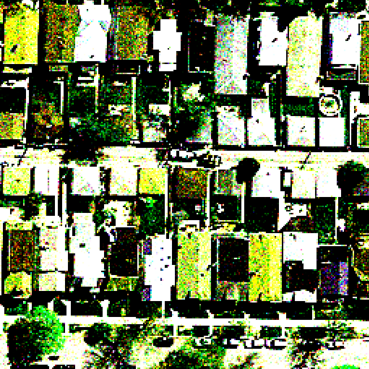
\includegraphics[width=.2\columnwidth]{images/centered.png}};
    
        \draw[arrow] (original) edge node[label] {1} (enhanced);
        \draw[arrow] (enhanced) |- ($(enhanced)+(0,-1.75)$) -| (crop1);
        \draw[arrow] (enhanced) |- ($(enhanced)+(0,-1.75)$) -| (crop2);
        \draw[arrow] (enhanced) |- ($(enhanced)+(0,-1.75)$) node[label] {2} -| (crop3);
        \draw[arrow] (crop1) |- ($(crop1)+(0,-1.25)$) node[label,left=10pt] {3} -| (noise);
        \draw[arrow] (noise) edge node[label] {4} (centered);
    \end{tikzpicture}
    
    \caption{The pre-processing pipeline consists of multiple steps. (1) The original image is enhanced. (2) It is then cropped into multiple patches. The patches are randomly flipped and rotated. (3) Noise is added and the colour of each patch is randomly modified. (4) Lastly, patches are centred per RGB channel. }
    \label{fig:processing_pipeline}
\end{figure}

\textbf{Image Enhancement}
Firstly, all images are enhanced. The goal of this step is to remove unnecessary information but leaving important information intact. We achieve this by first applying a Gaussian blurring filter to smooth all images. This removes small artefacts and colour variations without distorting the structure. The blurred images are then sharpened by applying a sharpening filter to amplify the crucial structures.

\textbf{Train-Time Augmentation}
In the second step, images from the training dataset are augmented. This yields a larger dataset with images of smaller size making the model more robust and more efficient. This step itself is split into two sub-steps: Patch Creation and Image Alteration. Patch Creation enlarges the dataset whereas Image Alteration makes it less prone to over-fitting by transforming the images in a random manner.

\textit{Patch Creation}: We experimented with several patch creation methods. The first method being no cropping at all. Images are left in their full size. Our second method crops the original image into five patches using a five-crop. This multiplies the size of the dataset by a factor of five with each patch containing mostly different information. Our third method crops the original image at a random location with random orientation. This approach has the advantage of multiplying the size of the dataset by an arbitrary factor.

\textit{Image Alteration}: The resulting patches or full-size images from the Patch Creation step are altered by random rotations in steps of 90 degrees. In addition, random flips are applied. These transformations are possible due to the nature of aerial imagery: The perspective reflects reality no matter its orientation.

\textbf{Noise Addition}
Train-Time Augmentation leads to multiple variants of the same original image. These variants differ from each other but can still contain similarities. These similarities and the size of the dataset, which we enlarged in the previous step but is still relatively small, carries the risk of over-fitting.

Hence, we apply random noise in the form of colour jitter and Gaussian noise to the patches in our third pre-processing step. Applying colour-jitter randomly varies the brightness, contrast, saturation, and hue of each patch. Adding Gaussian noise slightly distorts random pixels in the entire patch. Both mechanisms lead to a more robust model.

\textbf{Centering}
Lastly, the images are centred per RGB channel.


\subsection{Post-Processing}

The use of train-time augmentation also paves the way for test-time augmentation: Since the model was trained on patches, the test images need to be predicted in the same size too. Moreover, we experimented with morphological operators and the graph cut algorithm to remove undesired artefacts from the predictions.

\textbf{Test-Time Augmentation}
Images to be predicted are first cut into patches. This is performed in such a way that each patch overlaps with other patches. The patches are then predicted by the model resulting in multiple predictions for the same area of the original image.

We explored different methods to blend the predictions, depicted in Figure \ref{fig:test_time_augmentation}. The most straightforward one just picks one value. As a result, one patch covers the other patches resulting in sharp borders. Our second method takes the average of each overlapping value resulting in smoother transitions. However, the borders are still visible. Therefore, we introduced weights: Pixels close to the patch borders are weighted less than pixels in the centre. After applying the weights, overlapping patches are averaged. This approach smooths the borders even further.

\begin{figure}[h]
    \textit{Patch placement:}
    
    \vspace{5pt}
    
    
\includegraphics[width=.5\columnwidth]{images/patch_locations.png}
    
    \vspace{5pt}
    
    \textit{Blended patches:}
    
    \vspace{5pt}
    
    \centering
    \begin{subfigure}[t]{.3\columnwidth}
        \frame{
\includegraphics[width=\textwidth]{images/cover.png}}
        \caption{Cover}
        \label{fig:cover}
    \end{subfigure}
    \hfill
    \begin{subfigure}[t]{.3\columnwidth}
        \frame{
\includegraphics[width=\textwidth]{images/average.png}}
        \caption{Average}
        \label{fig:average}
    \end{subfigure}
    \hfill
    \begin{subfigure}[t]{.3\columnwidth}
        \frame{
\includegraphics[width=\textwidth]{images/weighted_average.png}}
        \caption{Weighted Average}
        \label{fig:weighted_average}
    \end{subfigure}
    
    \caption{The predicted patches are reassembled using different blend modes. In this illustration, four corner patches are blended together. (a) The cover blend mode picks one patch covering all other patches. (b) The average blend mode calculates the average of all overlapping pixels. (c) The weighted average blend mode weighs pixels closer to a patch border less and calculates the average of the overlapping weighted pixels.}
    \label{fig:test_time_augmentation}
\end{figure}


\textbf{Predicting}
We have used thresholding to convert the probability-based output of the segmentation model into the binary for submission. We have manually tested different values for this purpose in combination with various morphological operators such as morphological closing, erosion and dilation. In doing so, we were able to correct undesirable artefacts, or incorrect classification, in the output, such as small openings in the road segments. 

\textbf{Graph Cut}
Instead of thresholding, we also experimented with applying the graph cut algorithm \cite{Superroad2021} to classify the probabilities.
A graph is set up, where the probabilities and the LAB-color distance between neighbouring pixels act as edge weights. The resulting partition is used to divide all pixels into road or non-road.
For most cases, thresholding gives slightly better results.


\subsection{Implementation Details}
For our implementation, we rely on the high-performance Python framework PyTorch Lightning. We train all our models for 35 epochs with a learning rate of $0.001$, a batch size of $4$, and an Adam optimizer. For the loss function, we use a noise-robust dice loss which is an advanced dice loss that performs better. Furthermore, we use pre-trained weights from the ImageNet dataset \cite{dosovitskiy2020vit} for our TransUNet model.

For experimental executions and hyperparameter tuning, we used the python library Tune \cite{liaw2018tune}. In combination with Tensorboard, we were able to compare the loss and the accuracy of various hyperparameters variations efficiently. We particularly chose this library due to its performance on GPU and  ease of implementation.



\subsection{Other Lead}
A different lead, we explored early on, is the observation that a road network resembles a graph in many ways. Intersections can be interpreted as nodes and roads connecting them as straight edges. Curves could even be approximated by multiple consecutive edges. Thus, the idea popped up to implement a module, that transforms a list of edges, with a starting point, endpoint and thickness, into a road mask image. A network could be put in front of this edges-to-mask module that learns where the road edges lie, instead of attempting to interpret the pixels directly. After some time and experimenting, we hit a differentiability problem. This module is required to interpret values of the input tensor as indices in the output image. A road is drawn at indices, that are defined by values. As far as we were able to find out, this operation cannot guide a learning algorithm, as the gradients are conditionally set and not smooth. Further, training a network to find a list of edges from roads proves also to be a challenge in itself.




\section{Results}
The TransUNet architecture together with all improvements and data augmentations achieves a score of $0.876$.
We compare it to the Att UNet, R2 UNet and R2 Att UNet, that act as baselines \cite{DBLP:journals/corr/abs-1906-07160}. The Att UNet also incorporates the attention mechanism and provides interesting insight for comparison.  All augmentations, like pre- and post-processing methods, are also applied to all baselines. A summary of all final results is presented in Table \ref{tab:results}.

\textbf{Attention UNet:} This model \cite{oktay2018attention} has proved to consistently improve prediction accuracy across different datasets in the medical field. The model uses grid-based gating that allows attention coefficients to be more specific to local regions and applies soft-attention techniques.

\textbf{R2 UNet:} This model \cite{alom2018recurrent} combines U-Net, Residual Network, as well as Recurrent Convolutional Neural Network (RCNN) to gain several advantages in segmentation tasks. Tested with specific medical segmentation tasks the model has shown superior performances compared to U-Net. 

\setlength{\extrarowheight}{5pt}
\begin{table}[htbp]
\centering
   \begin{tabular}[c]{lll}
    \hline
    Method&Public&Private\\
    \hline
    UNet w/o pre/post & 0.843 & 0.934\\
    UNet & 0.859 & 0.923\\
    Att UNet & 0.865 & 0.934\\
    R2 UNet & 0.847 & 0.805\\
    R2 Att UNet & 0.847 & 0.803 \\
    \hline
    TransUNet w/o pre/post & 0.858 & 0.935 \\
    TransUNet & 0.876 & 0.931\\
    \hline
  \end{tabular}
  \caption{Performance evaluation and comparison}
  \label{tab:results}
\end{table}


\section{Discussion}
The initial intuition was, that in road images dependencies exist between far lying pixels of the same road and that Transformer would be able to capture this global context in the data. However, against our intuition, our compilation of different methods with the TransUNet as the core model can not significantly outperform any baselines. The other architectures all show similar results for both private and public scores. The pre- and post-processing steps, however, improved the score significantly and have helped enlarge the dataset and enhance training.


\section{Summary}
The presented work provided a promising demonstration of Transformers beyond medical image segmentation. 
We introduced the hybrid Transformer CNN model, TransUNet, to the problem of aerial road image segmentation. Together with various methods to increase the quality and quantity of the data, we attempted to improve the score.
Unfortunately, TransUNet seems to be not as effective for all computer vision problems. Their strong ability to capture global context does not lend itself to road segmentation from aerial images. Nonetheless, the project offered many insights and we were able to take a lot with us. 



\bibliographystyle{IEEEtran}
\bibliography{groupRosas-literature}
\end{document}
